\section{9. Deployment and component placement}

\begin{figure}[H]
\centering
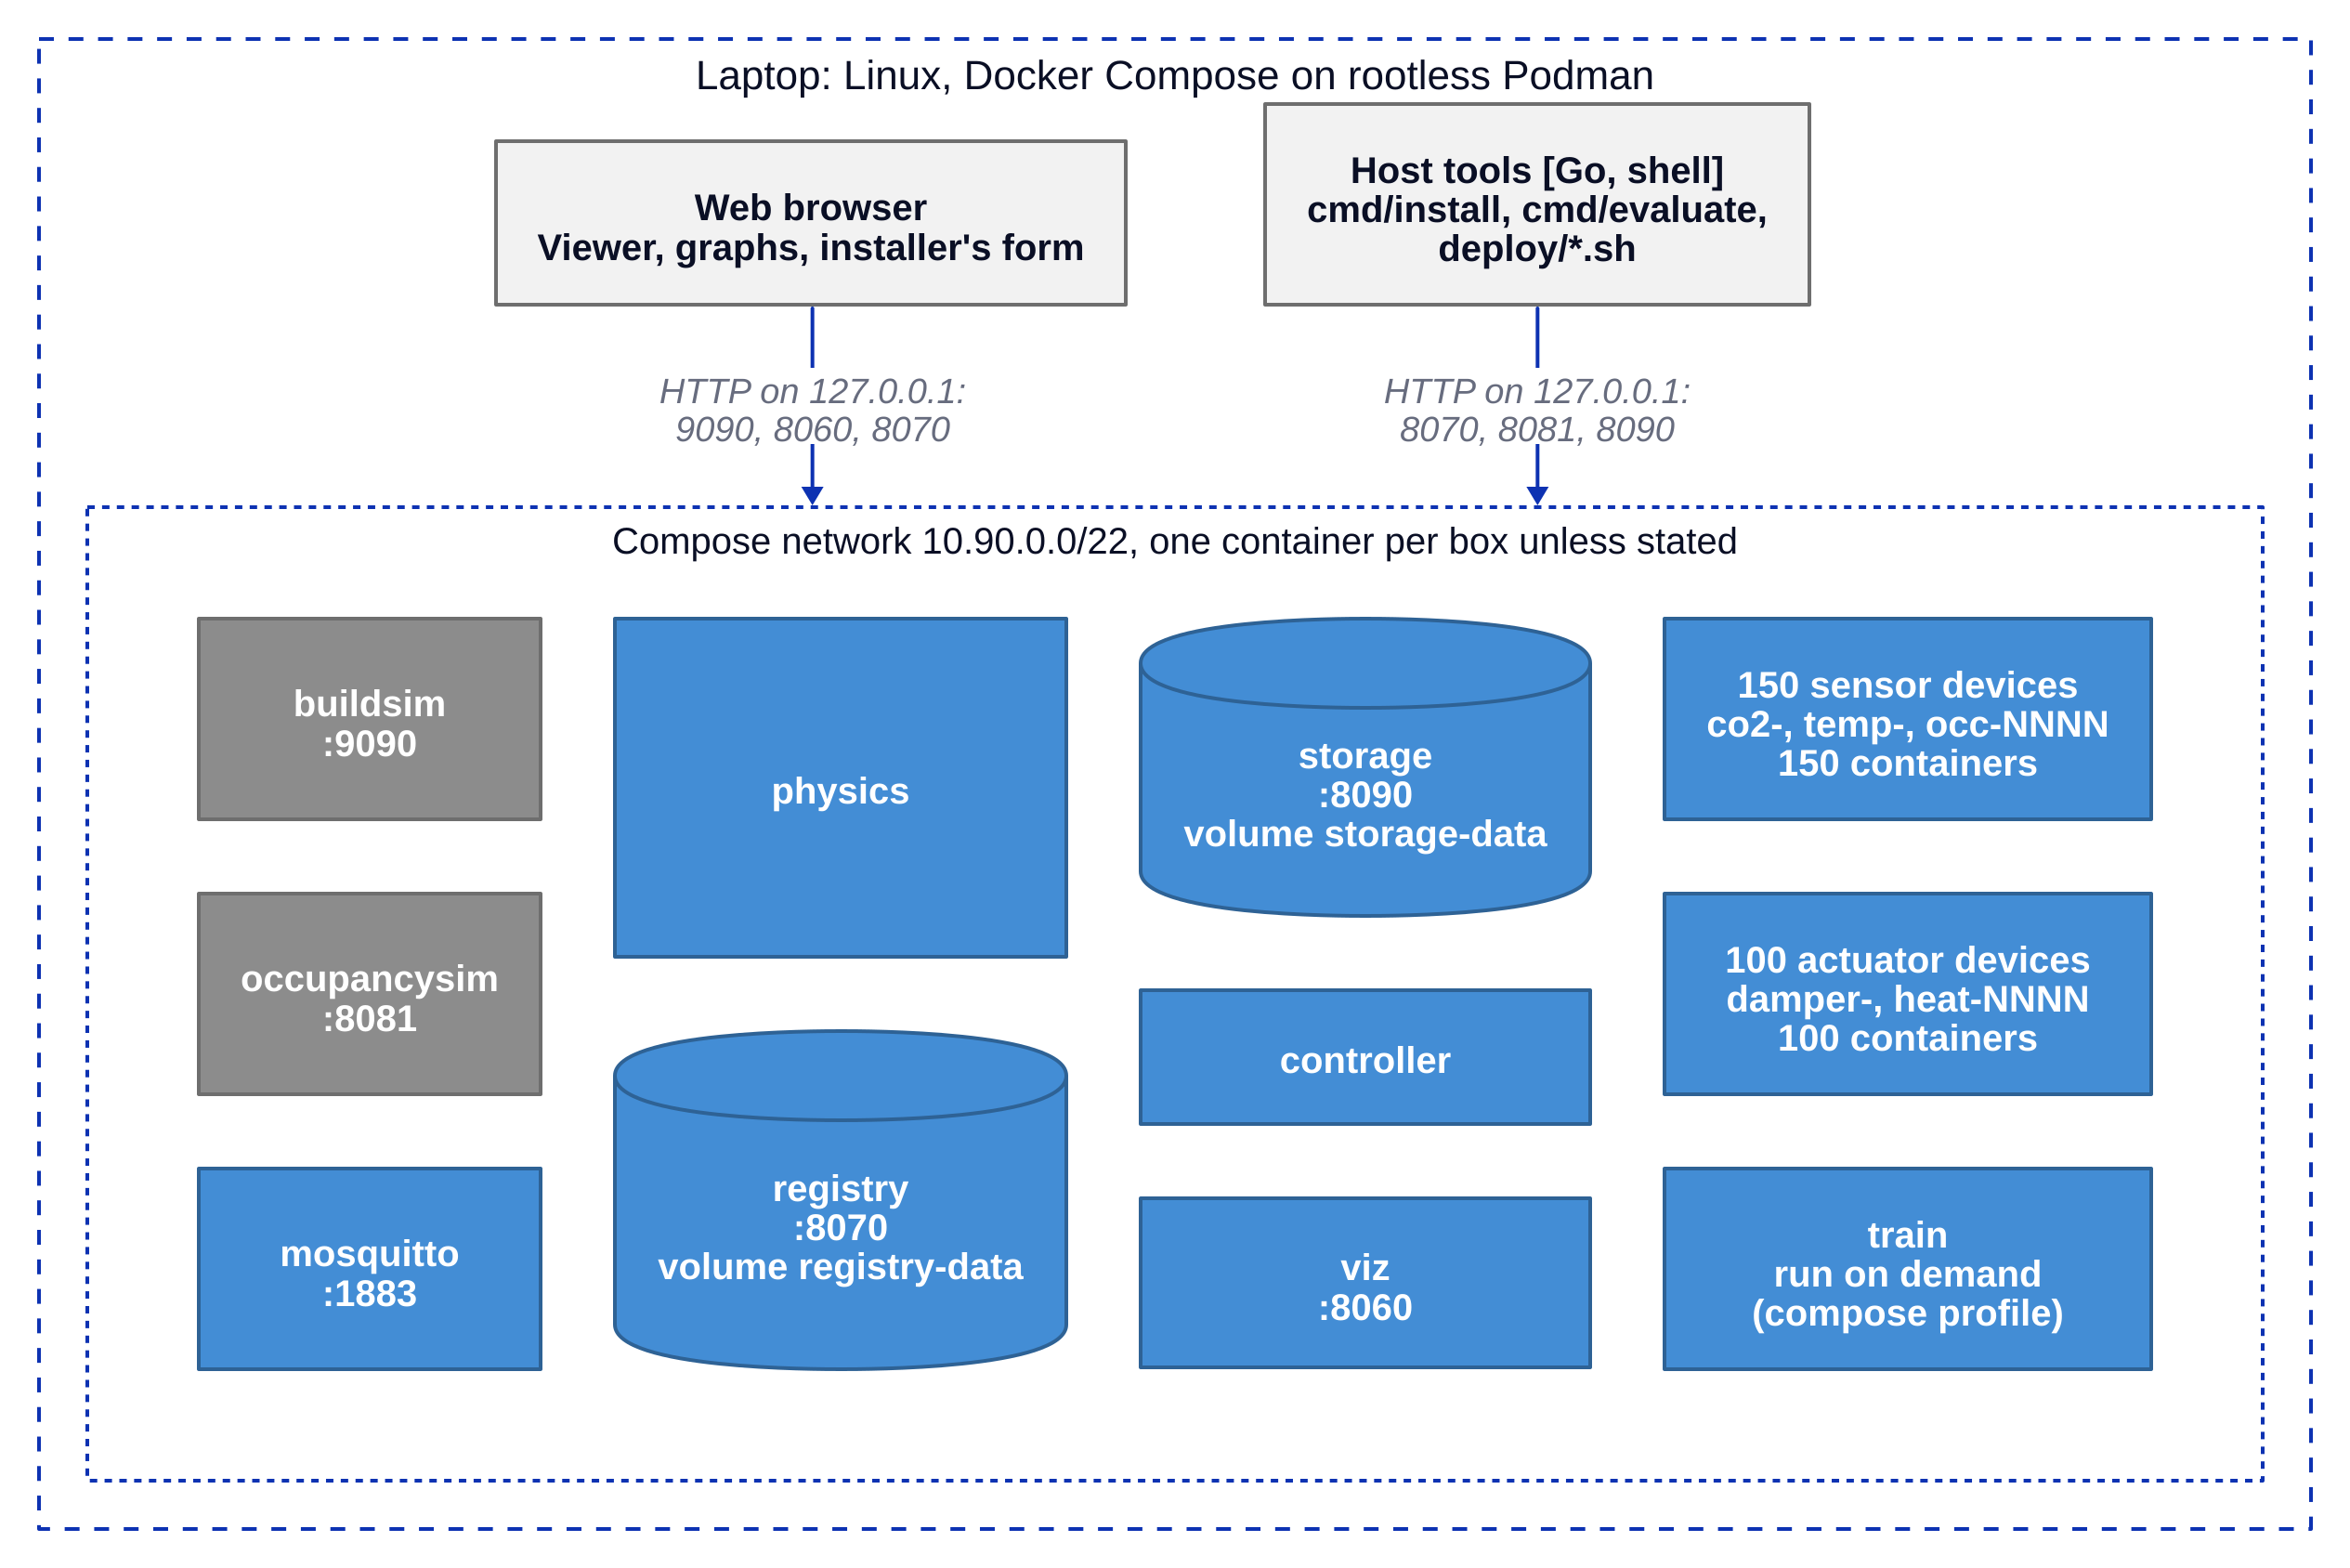
\includegraphics[width=0.86\linewidth]{figures/deployment.png}
\caption{Deployment. Everything runs on one laptop; the links between the
containers are those of Figures~\ref{fig:container}
and~\ref{fig:container-support}. Ports are published on 127.0.0.1 only.}
\label{fig:deployment}
\end{figure}

Everything runs on one laptop, as 258 containers under Docker Compose: the 8
services of \code{compose.yaml} and the 250 devices of the generated
\code{compose.devices.yaml}. Deployment is therefore about how the system is
cut into processes and what each cut buys, not about geography.

\textbf{Isolation.} Each container has one job and talks to the others only
through the interfaces of Section 5. No two share memory or files; the only
volumes are the registry's database and storage's run files, each used by one
container. A container can be stopped, started and replaced on its own, which
is what the fault tests of Section 10 do.

\textbf{Where each part would run in a real building.} The cut into containers
follows that question:
\begin{itemize}
\tightlist
\item \textbf{Sensor and actuator devices} are the hardware in the rooms. That
  is why they are one process each, why the safety limits live in the
  actuator, and why a device learns its room from a registry and not from a
  configuration file.
\item \textbf{The broker, the controller, the registry and storage} belong on
  a server in the building. The control loop must not depend on a connection
  to anywhere else, and a decision per room and minute needs no more than a
  small machine: the whole stack used about one CPU core at factor 60, which
  is sixty times real time.
\item \textbf{Training} is the only part that could move off-site. It is batch
  work, it is off the control path, and if its result never arrives the
  controller keeps the model it has, or runs reactively without one.
\item \textbf{The dashboard} can run anywhere that reaches the broker. It only
  reads.
\item \textbf{physics and occupancysim} would not exist. They stand in for the
  building and its people.
\end{itemize}

\textbf{What merging would cost.} Merging the devices into one process per
kind, which we built first, means one crash silences a kind of sensor in every
room. Merging the safety limits into the controller means they die with it.
Merging storage into the controller means the dashboard and the trainer read
the controller's files, which the course forbids and which ties three
lifetimes together.

\textbf{What one process per device costs.} 250 device containers are the
largest operational cost of the design, and they made the laptop, not our
code, the first limit (Section 11): Podman's keyring per container, the size of
the compose network, and the kernel's neighbour table all had to be raised
before 50 rooms would start. The compose network is a /22 for that reason.
On the development laptop (16 hardware threads) all containers together used
about one core at factor 60, started in about 40~s, and the 250 devices
registered in 26~s (2026-09-30). On a second laptop the same stack used about
1.2 cores and 1.7~GB of memory, started in 90~s and registered in 5~s
(2026-10-10).

\textbf{Operation.} \code{docker compose up -d} starts everything.
Devices start uncommissioned, so the installation list is registered once with
\code{cmd/install}; the registry's database is a volume, so this survives
restarts. \code{RUN\_ID} tags every record of an experiment and is set for the
whole stack at once. The policy is changed by restarting the controller alone.
